 %----------------------------------------------------------------------------------------
%	PACKAGES AND OTHER DOCUMENT CONFIGURATIONS
%----------------------------------------------------------------------------------------
\documentclass[paper=a4, fontsize=11pt]{scrartcl} % A4 paper and 11pt font size
\usepackage[T1]{fontenc} % Use 8-bit encoding that has 256 glyphs
\usepackage{fourier} % Use the Adobe Utopia font for the document - comment this line to return to the LaTeX default
\usepackage[english]{babel} % English language/hyphenation
\usepackage{amsmath,amsfonts,amsthm} % Math packages
\usepackage{lipsum} % Used for inserting dummy 'Lorem ipsum' text into the template
\usepackage{sectsty} % Allows customizing section commands
\allsectionsfont{\centering \normalfont\scshape} % Make all sections centered, the default font and small caps
\usepackage{fancyhdr} % Custom headers and footers
\usepackage[]{mcode}
\usepackage{amsmath}
\usepackage{graphics}
\usepackage{graphicx}
\newcommand{\norm}[1]{\left\lVert#1\right\rVert}


\pagestyle{fancyplain} % Makes all pages in the document conform to the custom headers and footers
\fancyhead{} % No page header - if you want one, create it in the same way as the footers below
\fancyfoot[L]{} % Empty left footer
\fancyfoot[C]{} % Empty center footer
\fancyfoot[R]{\thepage} % Page numbering for right footer
\renewcommand{\headrulewidth}{0pt} % Remove header underlines
\renewcommand{\footrulewidth}{0pt} % Remove footer underlines
\setlength{\headheight}{13.6pt} % Customize the height of the header

\numberwithin{equation}{section} % Number equations within sections (i.e. 1.1, 1.2, 2.1, 2.2 instead of 1, 2, 3, 4)
\numberwithin{figure}{section} % Number figures within sections (i.e. 1.1, 1.2, 2.1, 2.2 instead of 1, 2, 3, 4)
\numberwithin{table}{section} % Number tables within sections (i.e. 1.1, 1.2, 2.1, 2.2 instead of 1, 2, 3, 4)

\setlength\parindent{0pt} % Removes all indentation from paragraphs - comment this line for an assignment with lots of text

%----------------------------------------------------------------------------------------
%	TITLE SECTION
%----------------------------------------------------------------------------------------

\newcommand{\horrule}[1]{\rule{\linewidth}{#1}} % Create horizontal rule command with 1 argument of height

\title{	
\normalfont \normalsize 
\horrule{0.5pt} \\[0.4cm] % Thin top horizontal rule
\huge ECE 532 - Homework 6 \\ Iterative Algorithms for Regularized Least Square\\ % The assignment title
\horrule{2pt} \\[0.5cm] % Thick bottom horizontal rule
}

\author{Qihong Lu} % Your name
\date{\normalsize\today} % Today's date or a custom date

\begin{document}

\maketitle % Print the title

%----------------------------------------------------------------------------------------
%	PROBLEM 1
%----------------------------------------------------------------------------------------

\section*{Question1 Landweber convergence}
\textbf{Consider the landweber iteration: $ A \in \mathbb{R}^{mxn}, b \in \mathbb{R}^m$, and $A$ has full column rank. Let's begin the iteration with some initial $x_0$ and : }\\
$$x_{k+1} = x_k - \tau A^T (A x_k - b) \hspace{1cm} \text{for} \hspace{.2cm} k = 0, 1, 2, ...$$

\textbf{a) We expect it converge to $x_* = (A^T A)^{-1} A^T b$. Define the error as $e_k := x_k - x_*$. \\Rewrite $e_{k+1} = P e_k$ }


\begin{align*} 
e_{k+1} &= x_{k+1} - x_*	\\
&= x_k - \tau A^T (A x_k - b) - x_*	 \tag{definition of $x_k$}\\
&= e_k - \tau A^T (A x_k - b)	\tag{$e_k = x_k - x_*$}\\
&= e_k - \tau A^T A x_k + \tau A^T b		\\
&= e_k - \tau A^T A (e_k + x_*) + \tau A^T b		\tag{$x_k = e_k + x_*$}\\
&= e_k - \tau A^T A e_k - \tau A^T A x_* + \tau A^T b		\\
&= e_k - \tau A^T A e_k - \tau A^T A (A^T A)^{-1}A^T b + \tau A^T b	\tag{$x_* = (A^T A)^{-1}A^T b $}\\
&= e_k - \tau A^T A e_k - \tau A^T b + \tau A^T b		\tag{$A^T A (A^T A)^{-1} = I$}\\
&= e_k - \tau A^T A e_k	\\
&= (I - \tau A^T A) e_k	\\
\end{align*}

To summarize, 
$$e_{k+1}= P e_k \hspace{1cm} \text{where} \hspace{.2cm} P = I - \tau A^T A$$

\newpage
\textbf{b) Define the residual $r_k := A x_k - b$. Write $r_{k+1} = Q r_k$ }

\begin{align*} 
r_{k+1} &= A x_{k+1} - b		\\
&= A [x_k - \tau A^T (A x_k - b)] - b	\tag{$x_{k+1} = x_k - \tau A^T (A x_k - b)$}	\\
&= A x_k - \tau AA^T (A x_k - b) - b		\\
&= r_k - \tau AA^T (A x_k - b) 	 \tag{$r_k = A x_k - b$}	\\
&= r_k - \tau AA^T (A A^{-1}(r_k + b) - b) \tag{$x_k  = A^{-1}(r_k + b)$} \\
&= r_k - \tau AA^T r_k  \\
&= (I - \tau AA^T) r_k  \\
\end{align*}
To summarize, 
$$r_{k+1}= Q r_k \hspace{1cm} \text{where} \hspace{.2cm} Q = I - \tau AA^T$$\\\\









\textbf{c) Let ${\sigma_i}$ be the singular values of A. Show that when $0 < \tau < \frac{2}{\sigma_1^2}$, we have $ \underset{k \to \infty}{\lim} e_k = 0$}\\

First of all, assume A is full rank, I can use the economy SVD to rewrite $A^TA$. 
$$
A = U \Sigma V^T \implies A^TA = V \Sigma^2 V^T
$$

Now, let's consider the $k^{th}$ error: 
\begin{align*} 
e_1 &= P e_0	\\
e_2 &= P e_1	 = P^2 e_0	\\
\vdots \\
e_k &= P e_{k-1} = \dots = P^k e_0 \\
\end{align*} 

Since $P = I - \tau A^T A$, 
\begin{align*} 
e_k & = P^k e_0  \\ 
& = (I - \tau A^T A)^k e_0  \tag{$P = I - \tau A^T A$} \\ 
& = (I - \tau V \Sigma^2 V^T)^k e_0  \tag{$A^TA = V \Sigma^2 V^T$} \\ 
\end{align*} 



$$
I - \tau V \Sigma^2 V^T = 
\begin{bmatrix}
    1 & 0 & \dots  & 0 \\
    0 & 1 & \dots  & 0 \\
	\vdots & \vdots & \ddots & \vdots \\
    0 & 0 & \dots  & 1
\end{bmatrix} 
- \tau V
\begin{bmatrix}
    \sigma_{1}^2 & 0 & \dots  & 0 \\
    0 & \sigma_{2}^2 & \dots  & 0 \\
	\vdots & \vdots & \ddots & \vdots \\
	0 & 0 & \dots  & \sigma_{r}^2
\end{bmatrix} V^T 
= 
V
\begin{bmatrix}
    1- \tau \sigma_{1}^2 & 0 & \dots  & 0 \\
    0 & 1 - \tau \sigma_{2}^2 & \dots  & 0 \\
	\vdots & \vdots & \ddots & \vdots \\
	0 & 0 & \dots  & 1 - \tau \sigma_{r}^2
\end{bmatrix} V^T 
$$

Since $I - \tau V \Sigma V^T$ is in the form of an eigen-decomposition ($ABA^{-1}$ with B diagonal), we have that 
$$
(I - \tau V \Sigma^2 V^T)^k= 
V
\begin{bmatrix}
    1- \tau \sigma_{1}^2 & 0 & \dots  & 0 \\
    0 & 1 - \tau \sigma_{2}^2 & \dots  & 0 \\
	\vdots & \vdots & \ddots & \vdots \\
	0 & 0 & \dots  & 1 - \tau \sigma_{r}^2
\end{bmatrix}^k V^T 
= 
V
\begin{bmatrix}
    (1- \tau \sigma_{1}^2)^k & 0 & \dots  & 0 \\
    0 & (1 - \tau \sigma_{2}^2)^k & \dots  & 0 \\
	\vdots & \vdots & \ddots & \vdots \\
	0 & 0 & \dots  & (1 - \tau \sigma_{r}^2)^k
\end{bmatrix} V^T 
$$

To show that $ \underset{k \to \infty}{\lim} e_k = 0$, I need to show $P^k$ converges to the zero matrix.\\
P is diagonal, that means we need all diagonal entris to converge to zero. Namely, 
$$ \underset{k \to \infty}{\lim} (1 - \tau \sigma_{i}^2)^k = 0 \hspace{.5cm} \forall i $$ 
The k th power of $1 - \tau \sigma_{1}^2$ converge to zero if $|1 - \tau \sigma_{1}^2| < 1$, which means that: 
\begin{align*}
-1< 1 - \tau \sigma_{1}^2 < 1 	\\ 
-2<  - \tau \sigma_{1}^2 < 0 	\\ 
0<  \tau \sigma_{1}^2 < 2 	\\ 
0 < \tau  < \frac{2}{\sigma_{1}^2} \\ 
\end{align*}
Where $\sigma_{1} $ is the largest singular value of A. 

So we require $0 < \tau  < \frac{2}{\sigma_{1}^2}$ for the error to converge to 0. \\\\\\




\textbf{alternative idea: show that $  \underset{k \to \infty}{\lim} \|P\|^k = 0 $}

By the property of the norm operator $\|x\| = 0 \implies x = 0 $\\
We have that $\underset{k \to \infty}{\lim} \|P\|^k = 0 \implies \underset{k \to \infty}{\lim} P^k = 0$. So we just need to show $\|P\| < 1$  

$$
\|P\| = \| I - \tau V \Sigma^2 V^T \| 
= 
\norm{  
I - \tau V
\begin{bmatrix}
    \sigma_{1}^2 & 0 & \dots  & 0 \\
    0 & \sigma_{2}^2 & \dots  & 0 \\
	\vdots & \vdots & \ddots & \vdots \\
	0 & 0 & \dots  & \sigma_{r}^2
\end{bmatrix} 
V^T }
=
\norm{  
\begin{bmatrix}
    1- \tau \sigma_{1}^2 & 0 & \dots  & 0 \\
    0 & 1 - \tau \sigma_{2}^2 & \dots  & 0 \\
	\vdots & \vdots & \ddots & \vdots \\
	0 & 0 & \dots  & 1 - \tau \sigma_{r}^2
\end{bmatrix}}
=  |1- \tau \sigma_{1}^2|
$$

In the step where I took out $V$ and $V^T$, I was using the fact that orthogonal transformation doesn't not change the norm. Because A is full column rank, $V$ is an orthogonal under the economy SVD. \\

Similarly, we still require $|1- \tau \sigma_{1}^2| < 1$, which tells us that $0 < \tau  < \frac{2}{\sigma_{1}^2}$. 




\newpage
\textbf{d) Show that if A is rank-deficient and $x_0 = 0$, then the landweber iteration converges to the minimun norm solution. }\\ 

The error is
\begin{align*}
e_k &:= x_k - x_* 		\\
\Rightarrow  x_k &= e_k + x_* = e_k + A^\dagger b
\end{align*}

And I need to show that the error goes to zero as k goes to infinity. 

A is rank deficient, we use the full sized SVD: $A = U \Sigma V^T$. Then $A^T A = V \Sigma^2 V^T$ where V is orthogonal. \\

Again, $e_k = P^k e_0$. But $P$ goes to zero for similar reason stated previous. So $e_k$ would goes to zero as k goes to infinity. \\

The limit of solution: 
\begin{align*}
\underset{k \to \infty}{\lim} x_k &= \underset{k \to \infty}{\lim} (A^\dagger b + e_k) \\
& = A^\dagger b + \underset{k \to \infty}{\lim} e_k \\
& = A^\dagger b  \tag{$\underset{k \to \infty}{\lim} e_k =0$}
\end{align*}

And $A^\dagger b $ is the minimal norm solution of the least square problem when A is rank deficient. 

%----------------------------------------------------------------------------------------
%	PROBLEM 2
%----------------------------------------------------------------------------------------
\newpage
\section*{Question2 Data Fitting vs. Sparsity Trade off}

\textbf{a) Implement ISTA to solve lasso}


Just to show the the implementat works, here's the error on the training set, which goes to zero. The algorithm stops when the 2 norm of the change of beta  is smaller than 0.001. 

\begin{center}
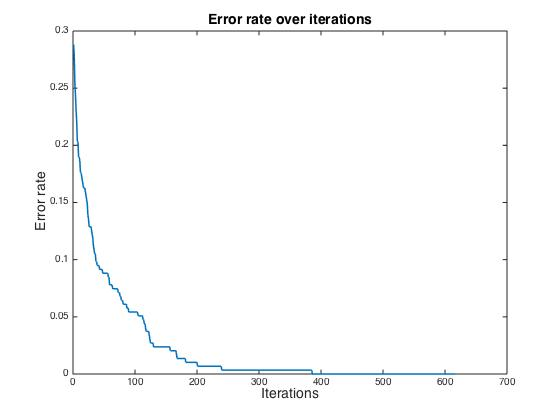
\includegraphics[scale=.5]{hw6_2a_error.jpg}
\end{center}

Here's the main script
\begin{lstlisting}
clear all; close all; clc;
% read data
load('BreastCancer.mat')

% set parameter, lambda, learning rate, ...
tau = .9/ norm(X,2)^2;
lambda = .1;

[beta, record] = lasso_lsta(X, y, lambda, tau, 1);

\end{lstlisting} 

And here's the code for iterative method for lasso. 
\begin{lstlisting}
%% iterative soft thresholding to lasso
function [beta, record] = lasso_lsta(X, y, lambda, tau, display)

%% set some parameters
maxIter = 50000;   % maxiteration that the program will run
tolerance = 1e-3;

%% compute things that need to be computed many times
[m,n] = size(X);
tau_XTy = tau * X' * y;
tau_XTX = tau * X' * X;
% preallocate
beta = zeros(n,1);
if display
    fprintf('iter\taccuracy\tdiff_beta\tnnz\n');
end
for i = 1 : maxIter;
    %% update weight
    Z = beta(:,i) - tau_XTX * beta(:,i) +  tau_XTy;
    beta(:,i+1) = sign(Z) .* max((Z - 2*lambda*tau), 0);
    
    %% Performance monitoring
    % compute change in beta
    diff = norm(beta(:,i+1) - beta(:,i));
    % nnz for the updated beta
    nnz = n-numZeros(beta(:,i+1));
    % error of the updated beta
    record.accuracy(i) = sum(sign(X * beta(:,i+1)) == y) / m;
    % print the performance
    if display
        fprintf('%4d%12.4f %16.4f %10d\n', i, record.accuracy(i), diff, nnz);
    end
    
    %% stopping criterion
    if diff < tolerance
        break;
    end
end

% plot the performance
if display
    plotError(1-record.accuracy)
end
end

%% function for plotting the errors
% input: error rate over iterations
function plotError(error)
FZ = 14;
plot(error, 'linewidth', 1.5)
title('Error rate over iterations', 'fontsize', FZ)
xlabel('Iterations', 'fontsize', FZ)
ylabel('Error rate', 'fontsize', FZ)
end

%% check the number of non zero betas
% input
function [nz] = numZeros(beta)
tolerance = 1e-6;
% calculate number of "zeros"
nz = sum(abs(beta) <= tolerance);
end

\end{lstlisting}



\newpage
\textbf{b) Use the 1st 100 patients, plot the trade-off (residual against the 1 norm of beta) of the training data}\\

Here's the plot visualizing the trade off between the training set residual and the norm. 
\begin{center}
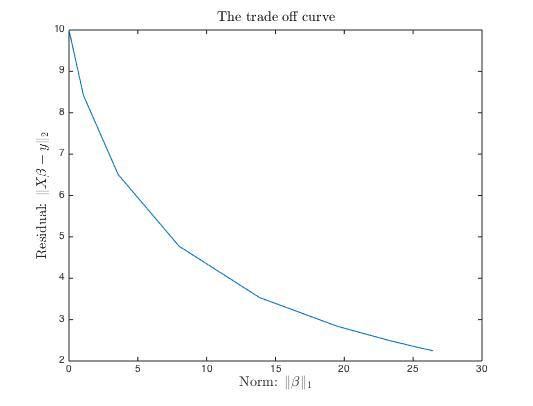
\includegraphics[scale=.5]{hw6_2b_tradeoff.jpg}
\end{center}

I used 20 lambda values, chose from logarithmically spaced from $10^{-4}$ to $10^{4}$ with the matlab command: logspace(-4,4,20). On the plot above, the lambda value is decreasing from the left to the right, as showed in class. \\

On the left hand side of the graph, the lambda is huge, and lasso is emphasize minimizing the 1 norm of $\beta$, so $\|\beta\|_1$ is close to zero. However, the model is less good at minimizing the residual. \\

On the right hand side of the graph, the lambda is tiny. So having large $\|\beta\|_1$ is not a "concern" for the lasso. Consequently, the $\|\beta\|_1$  is very large. However, the benefit is that the lasso can concentrate on minizing the residual, so $\| X\beta - y \|_2$ is very small on the right hand side. 

\newpage
\textbf{c) Error against sparsity }\\ 

Here's the plot visualizing the trade off between the training set classification error and the sparsity, defined as the number of non-zero beta values.\\ 

Again, I used 20 lambda values, chose from logarithmically spaced from $10^{-4}$ to $10^{4}$ with the matlab command: logspace(-4,4,20). On the plot above, the lambda value is decreasing from the left to the right, as showed in class. \\

\begin{center}
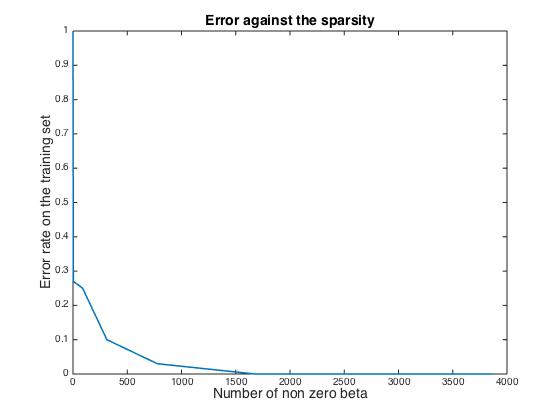
\includegraphics[scale=.5]{hw6_2c_err_spar.jpg}
\end{center}

On the left hand side of the graph, the lambda is huge, so lasso tried really hard to minizing the norm of beta. It tried so hard that the classification error becomes $100\%$, although the norm of beta becomes 0. It is good at minimizing the norm, but this is not a very useful classifier. \\ 

On the right hand side of the graph, the lambda is tiny. Lasso has no pressure of about the norm of the beta at all, so the number of non-zero beta is big. However, since lasso can fully focused on minimizing the classification error, the error goes to zero. 

\newpage
Here's the code for 2b and 2c. 
The lasso function is attached previously so I am not attaching it again. 
\begin{lstlisting}
% initialization
clear all; close all; clc;
load('BreastCancer.mat')

% set some parameters
numLambdas = 20;
LAMBDAS = flip(logspace(-4,4,numLambdas));
trainSize = 100;

% subset the data
Xtrain = X(1:trainSize,:);
ytrain = y(1:trainSize,:);

% set parameter, lambda, learning rate, ...
tau = .9/ norm(X,2)^2;

%% compute the trade off
for i = 1 : numLambdas
    fprintf('%d\n',i);
    %% fit a lasso model for a particular lambda
    [beta, record] = lasso_lsta(Xtrain, ytrain, LAMBDAS(i), tau, false);
    
    %% compute the performance
    % performance on the training data
    residual(i) = norm(Xtrain * beta(:,end) - ytrain,2);
    accuracy(i) = record.accuracy(end);
    % beta norm 
    norm_beta(i) = norm(beta(:,end),1);
    % nonzero betas
    nnz(i) = record.nonZeroBetas;
end

% plot the residual-norm trade off 
plot(norm_beta, residual, 'linewidth', 1.5)
FZ = 14;
title('The trade off curve','fontsize', FZ)
xlabel('Norm: $\|\beta\|_1$','Interpreter','LaTex', 'fontsize', FZ)
ylabel('Residual: $\|X \beta - y\|_2$','Interpreter','LaTex', 'fontsize', FZ)

% plot the error-sparsity trade off 
plot(nnz, 1-accuracy, 'linewidth', 1.5)
title('Error against the sparsity','fontsize', FZ)
xlabel('Number of non zero beta','fontsize', FZ)
ylabel('Error rate on the training set','fontsize', FZ)
\end{lstlisting}


\newpage
\textbf{d) The trade off curves on the test set}
\begin{center}
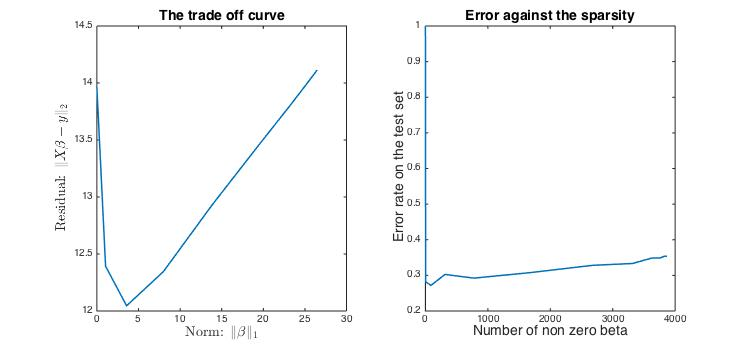
\includegraphics[scale=.6]{hw6_2d_tradeoffs.jpg}
\end{center}

On the left, I am plotting the residual-norm trade off. On the right, I am plotting the error-sparsity trade off. Now, the residual and error were computed using the test set, the choise of lambda values, stopping criterion are the same as previous problems. \\

For residual-norm trade off curve, $\|\beta\|_1$ follows the trend I saw in the training data. Namely, $\|\beta\|_1$ is huge for small lambda, and $\|\beta\|_1$ is small for huge lambda. However, the residual on test set shows a different patterns from the residual on the training set. Based on the convex shape of the trade off curve, we can see that tiny  lambda didn't do well on minimizing the test set residual, whereas a lambda of an intermediate value genenearlized well on the unseen test set data. One probably reason is that if we don't regularize at all (corresponds to tiny lambda), the lasso weights choise is more suspectible to the noise, which results in bad performance. \\

For the error-sparsity trade off, the number of non-zero $\beta$ follows the same patterns. The error on the test set has a different patterns from the error rate on the training set. For large lambda, the error is very high. Because the model is too focused on minimizing the norm of $\beta$, so it didn't do well on minizing the error. However, when the lambda become very small, the error didn't go to zero. Actually, when lambda become small enough, the error is no longer decreasing. So there might be an upper limit for the generalization, and it is hard to be perfect. 

\newpage
Here's the code for 2d. 
\begin{lstlisting}
% initialization
clear all; close all; clc;
load('BreastCancer.mat')
[m] = length(y);
% set some parameters
numLambdas = 20;
LAMBDAS = flip(logspace(-4,4,numLambdas));
trainSize = 100;
trainIdx = false(m,1);
trainIdx(1:trainSize) = 1;

% subset the data
Xtrain = X(trainIdx,:);
ytrain = y(trainIdx);
Xtest = X(~trainIdx,:);
ytest = y(~trainIdx);

% set parameter, lambda, learning rate, ...
tau = .9/ norm(X,2)^2;

%% compute the trade off
for i = 1 : numLambdas
    %% fit a lasso model for a particular lambda
    [beta, record] = lasso_lsta(Xtrain, ytrain, LAMBDAS(i), tau, false);
    
    %% compute the performance
    % performance on the training data
    prediction = Xtest * beta(:,end);
    residual(i) = norm(prediction - ytest,2);
    accuracy(i) = sum(sign(prediction) == ytest) / (m - trainSize);
    % beta norm 
    norm_beta(i) = norm(beta(:,end),1);
    % nonzero betas
    nnz(i) = record.nonZeroBetas;
end
%% plot the performance 
% plot the residual-norm trade off 
subplot(1,2,1)
plot(norm_beta, residual, 'linewidth', 1.5)
FZ = 14;
title('The trade off curve','fontsize', FZ)
xlabel('Norm: $\|\beta\|_1$','Interpreter','LaTex', 'fontsize', FZ)
ylabel('Residual: $\|X \beta - y\|_2$','Interpreter','LaTex', 'fontsize', FZ)
% plot the error-sparsity trade off 
subplot(1,2,2)
plot(nnz, 1-accuracy, 'linewidth', 1.5)
title('Error against the sparsity','fontsize', FZ)
xlabel('Number of non zero beta','fontsize', FZ)
ylabel('Error rate on the test set','fontsize', FZ)


\end{lstlisting}






\newpage
\textbf{e) Compare ridge and lasso}

\begin{center}
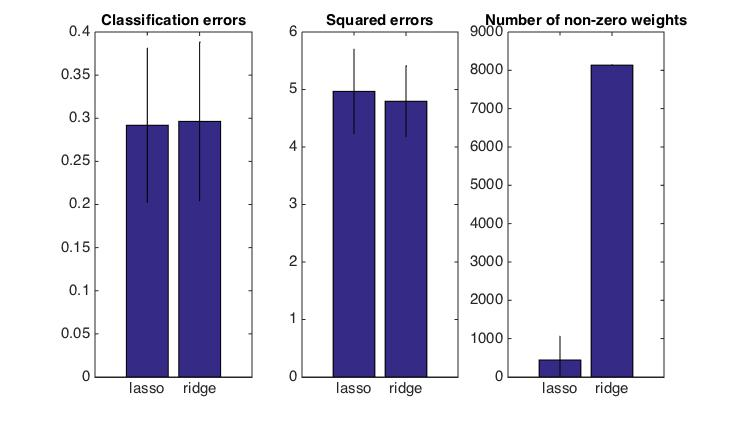
\includegraphics[scale=.5]{hw6_2e_comparel1l2.jpg}
\end{center}

Here I provide the some comparison of the classfication performance, measured by the mean classification error and the mean square error, and the sparsity, measured by mean number of non-zero weights. The error bars indicates one standard deviation. \\

For the classification error and square error, lasso and ridge regression performed similarly (the plot on the left and the middle). However, lasso used much less features to do so. In some sense, we can interpret the result as lasso achieve similar performance as the ridge regression with much less features. So in this case, the solutions provided by lasso is going to be more interpretable. Therefore, I prefer lasso. 

\newpage

Here's the matlab code I used to compare lasso vs. ridge
\begin{lstlisting}
% initialization
clear all; close all; clc;
load('BreastCancer.mat')
rng(1)

% set some parameters
[m,n] = size(X);
numLambdas = 20;
LAMBDAS = flip(logspace(-4,4,numLambdas));
tau = .9/ norm(X,2)^2;
K = 10;

%% final hold out set
% generate CV indices block for the final hold out set
CVIDX = crossvalind('Kfold', m, K);
CVB = false(m,K);
for k = 1 : K
    CVB(CVIDX == k,k) = true;
end

%% hold out 1 chuck of the data as the final test set
% k from 1 to 10
LASSO_BEST = cell(K,1);
RIDGE_BEST = cell(K,1);
for k = 1:K
    finalHoldoutIdx = CVB(:,k);
    Xtune = X(~finalHoldoutIdx, :);
    ytune = y(~finalHoldoutIdx);
    Xfinal = X(finalHoldoutIdx, :);
    yfinal = y(finalHoldoutIdx);
    
    %% set up CV block for the training set (weight search)
    % generate CV indices block
    CVIDX_b = crossvalind('Kfold', m - length(yfinal), K-1);
    CVB_b = false(m - length(yfinal), K-1);
    for kk = 1 : K-1
        CVB_b(CVIDX_b == kk, kk) = true;
    end
    
    %% inner cross-validation
    for kk = 1 : K-1
        
        % split training vs. test data
        testSetIdx = CVB_b(:,kk);
        Xtrain = Xtune(~testSetIdx, :);
        ytrain = ytune(~testSetIdx);
        Xtest = Xtune(testSetIdx, :);
        ytest = ytune(testSetIdx);
        
        %% loop over all values of regularization parameter lambda
        % set learning rate
        for l = 1 : numel(LAMBDAS)
            fprintf('%d - %d - %d \n', k, kk, l);
            lambda = LAMBDAS(l);
            % fit lasso model
            [tempbeta, ~] = lasso_lsta(Xtrain, ytrain, lambda, tau, 0);
            lasso.beta(:,l) = tempbeta(:,end);
            lasso.lambda(l) = lambda;
            lasso.accuracy(l) = sum(sign(Xtest * lasso.beta(:,l)) == ytest) / length(ytest);
            % fit ridge model
            [tempbeta, ~] = ridge_iter(Xtrain, ytrain, lambda, tau, 0);
            ridge.beta(:,l) = tempbeta(:,end);
            ridge.lambda(l) = lambda;
            ridge.accuracy(l) = sum(sign(Xtest * ridge.beta(:,l)) == ytest) / length(ytest);
        end
        
        %% find the best beta and the associated parameter
        % lasso
        bestIdx = find(lasso.accuracy == max(lasso.accuracy),1);
        LASSO_BEST{k}.beta(:,kk) = lasso.beta(:,bestIdx);
        LASSO_BEST{k}.lambda(kk) = lasso.lambda(bestIdx);
        % ridge
        bestIdx = find(ridge.accuracy == max(ridge.accuracy),1);
        RIDGE_BEST{k}.beta(:,kk) = ridge.beta(:,bestIdx);
        RIDGE_BEST{k}.lambda(kk) = ridge.lambda(bestIdx);
        
    end
    
    %% compute the performance on the final hold out set 
    for kk = 1 : K-1
        prediction = Xfinal * LASSO_BEST{k}.beta(:,kk);
        LASSO_BEST{k}.diff(kk) = norm(prediction - yfinal,2); 
        LASSO_BEST{k}.accuracy(kk) =  sum(sign(prediction) == yfinal)/length(yfinal);
        
        prediction = Xfinal  * RIDGE_BEST{k}.beta(:,kk);
        RIDGE_BEST{k}.diff(kk) = norm(prediction - yfinal,2); 
        RIDGE_BEST{k}.accuracy(kk) =  sum(sign(prediction) == yfinal)/length(yfinal);
    end
end

\end{lstlisting}

\end{document}